\documentclass{article}%
\usepackage[T1]{fontenc}%
\usepackage[utf8]{inputenc}%
\usepackage{lmodern}%
\usepackage{textcomp}%
\usepackage{lastpage}%
\usepackage{authblk}%
\usepackage{graphicx}%
%
\title{Introduction of 65 kDa Antigen of Mycobacterium tuberculosis to Cancer Cells Enhances Anti{-}Tumor Effect of BCG Therapy}%
\author{Anthony Russo}%
\affil{Department of Veterinary Medicine, School of Veterinary Medicine, National Taiwan University, Taipei, Taiwan, R.O.C., Department of Surgery, Mackay Memorial Hospital, Taipei, Taiwan, R.O.C., Research Institute for Children, Children's Hospital, New Orleans, LA, USA}%
\date{01{-}01{-}2012}%
%
\begin{document}%
\normalsize%
\maketitle%
\section{Abstract}%
\label{sec:Abstract}%
Advertisement\newline%
Within the past two months we have seen quite a bit of Bacillus cereuse activity.\newline%
First we saw the media discussing the break in the spread of Bacillus forylurea, Bacillus cereuse. This has seemed to support the hypothesis that the disease had actually been pushed back to the Central Valley in order to open up a container for Bacillus forylurea to enter the central valley.\newline%
Then we heard the story that Bacillus propagates through sea stone also known as sea cucumbers, which somehow still do infiltrate the Central Valley. This seems like a further evidence of Bacillus forylurea, because it is a little known fact that sea cucumbers do not grow at the same time in the Central Valley as in southern California.\newline%
The last article was about a problem with Bacillus as it is called in the veterinary community. The article discusses the history of the disease and the problem that it was growing by season. It is doubtful that the recent situation has happened because of the volume of Bacillus forylurea in the Central Valley, but rather by the nature of the disease itself. The reason that Bacillus forylurea has been spreading is that it is a very difficult disease to remove. It can hard to remove with heat and light. Even a vaccine for the disease can only remove Bacillus for two to three days.\newline%
Now we have seen a virus spreading like wild fire of Bacillus forylurea. This is called Bacillus rutiformis. There are many different strains of RUT in San Diego, including Caius rutiformis, Bacillus sigmundus, and this one called Bacillus krum.\newline%
So far the research in RUT has not shown that the spread of RUT is driven by Bacillus forylurea, which tells us something.\newline%
So why have conditions become so unstable and stable recently in the San Joaquin Valley?\newline%
One theory is that we are experiencing a new eruption of large effluent produced by our natural water bodies. Plants growing in these water bodies have been able to use the nutrients from the warm lake water as a means to colonize large areas of land and due to the drought we are in, many are flooding land areas and large swaths of open ground. This has been known for a while but to see the impacts, including the infiltration of large amounts of RUT, is shocking to those not familiar with our agricultural roots.\newline%
One area in the Sierra Nevada, the Del Monte Gulch at Yuba County, has been under water for a very long time. The water was once sourced from the nearby wetland salt deposits in the Sierra Nevada and when the water levels were low in the Del Monte Gulch, there were always enough plants to support the desert development in this area.\newline%
In fact, the Del Monte Gulch survived the drought in such a way that a vast plant canopy of bacillus cereuse grows right below the soil. This increased water levels in the Del Monte Gulch has resulted in too many plants competing for the same water, more fire activity in that area, and water rates that in the rest of the valley are unlikely to return to the pre{-}drought levels.

%
\subsection{Image Analysis}%
\label{subsec:ImageAnalysis}%


\begin{figure}[h!]%
\centering%
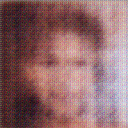
\includegraphics[width=150px]{500_fake_images/samples_5_207.png}%
\caption{A Close Up Of A Person Holding A Cell Phone}%
\end{figure}

%
\end{document}